\section{Mechanical packaging}\label{sec:mechanical}

The mechanical concept is a headless, parametric FreeCAD script, \texttt{mech/concept/speaker\_concept.py}. It writes the assembly (FCStd and STEP, with one named solid per part), STL files for every part, PCB outlines as DXF/SVG and a \texttt{report.json} containing volumes, an interference matrix and clearances. Every number below can be regenerated after a parameter change. The views were rendered with pyvista \src{docs/mech_envelope.md}. The parts are a packaging concept, not yet print-ready.

\begin{figure}[htbp]
\centering
\begin{subfigure}[t]{0.49\linewidth}\centering
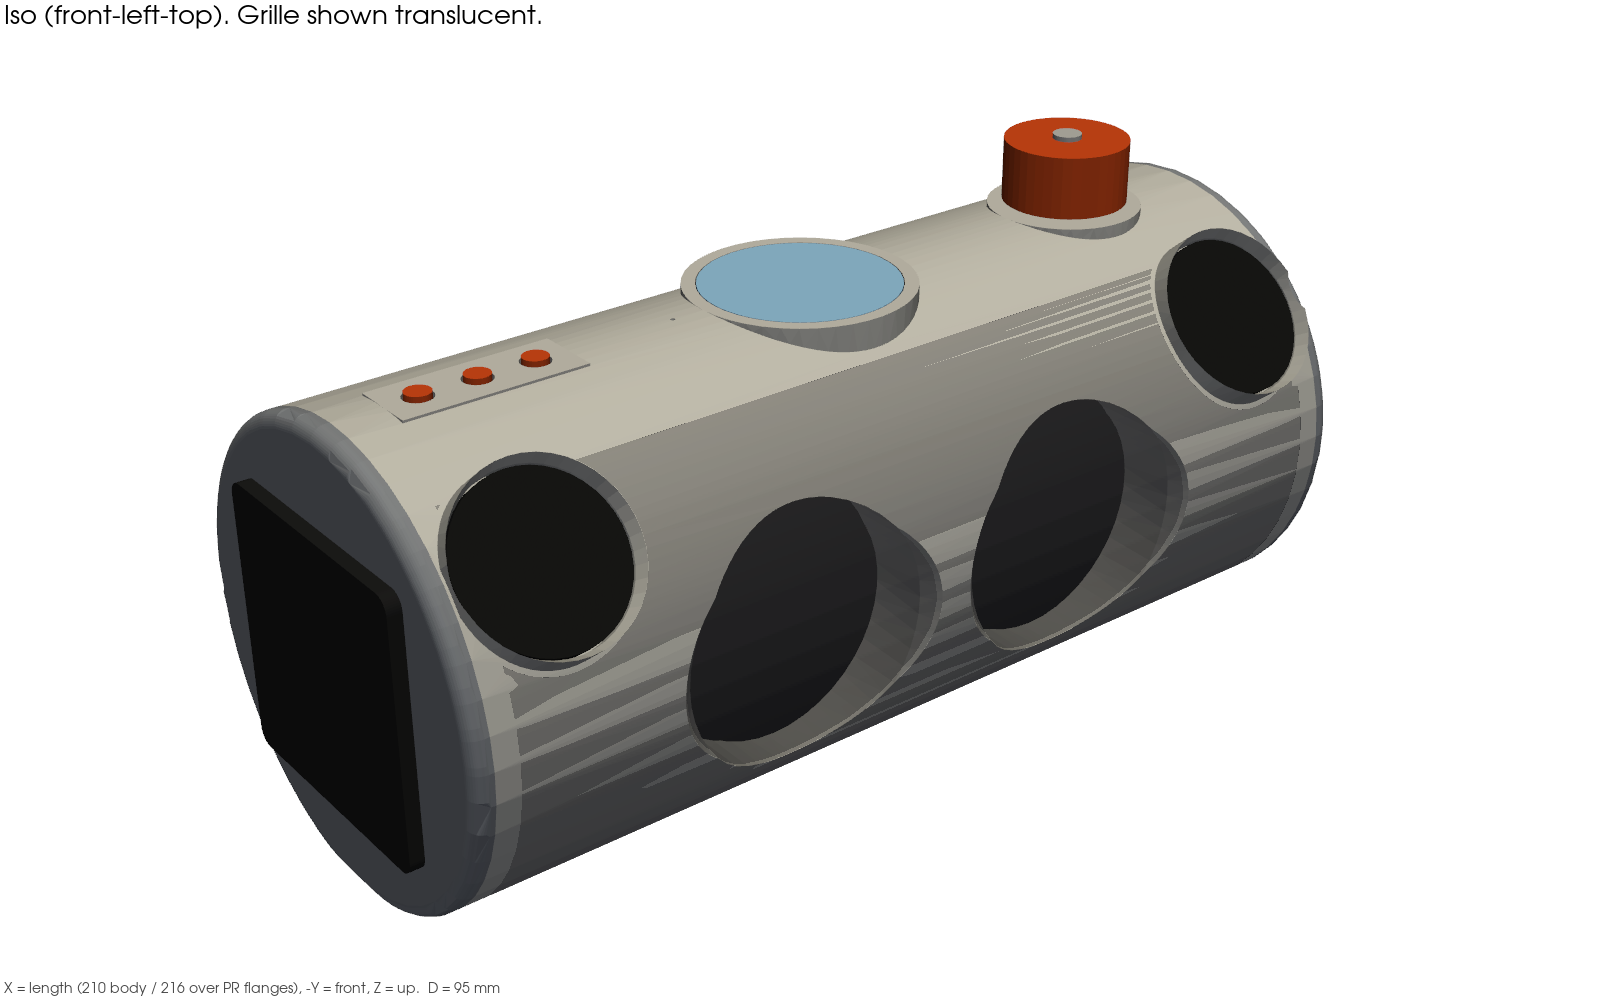
\includegraphics[width=\linewidth]{view_iso.png}
\caption{Iso view: the Ø\qty{95}{\milli\metre} capsule with grille, tweeter bosses on the front shoulders, display and knob on top, and a PR on each end cap.}
\end{subfigure}\hfill
\begin{subfigure}[t]{0.49\linewidth}\centering
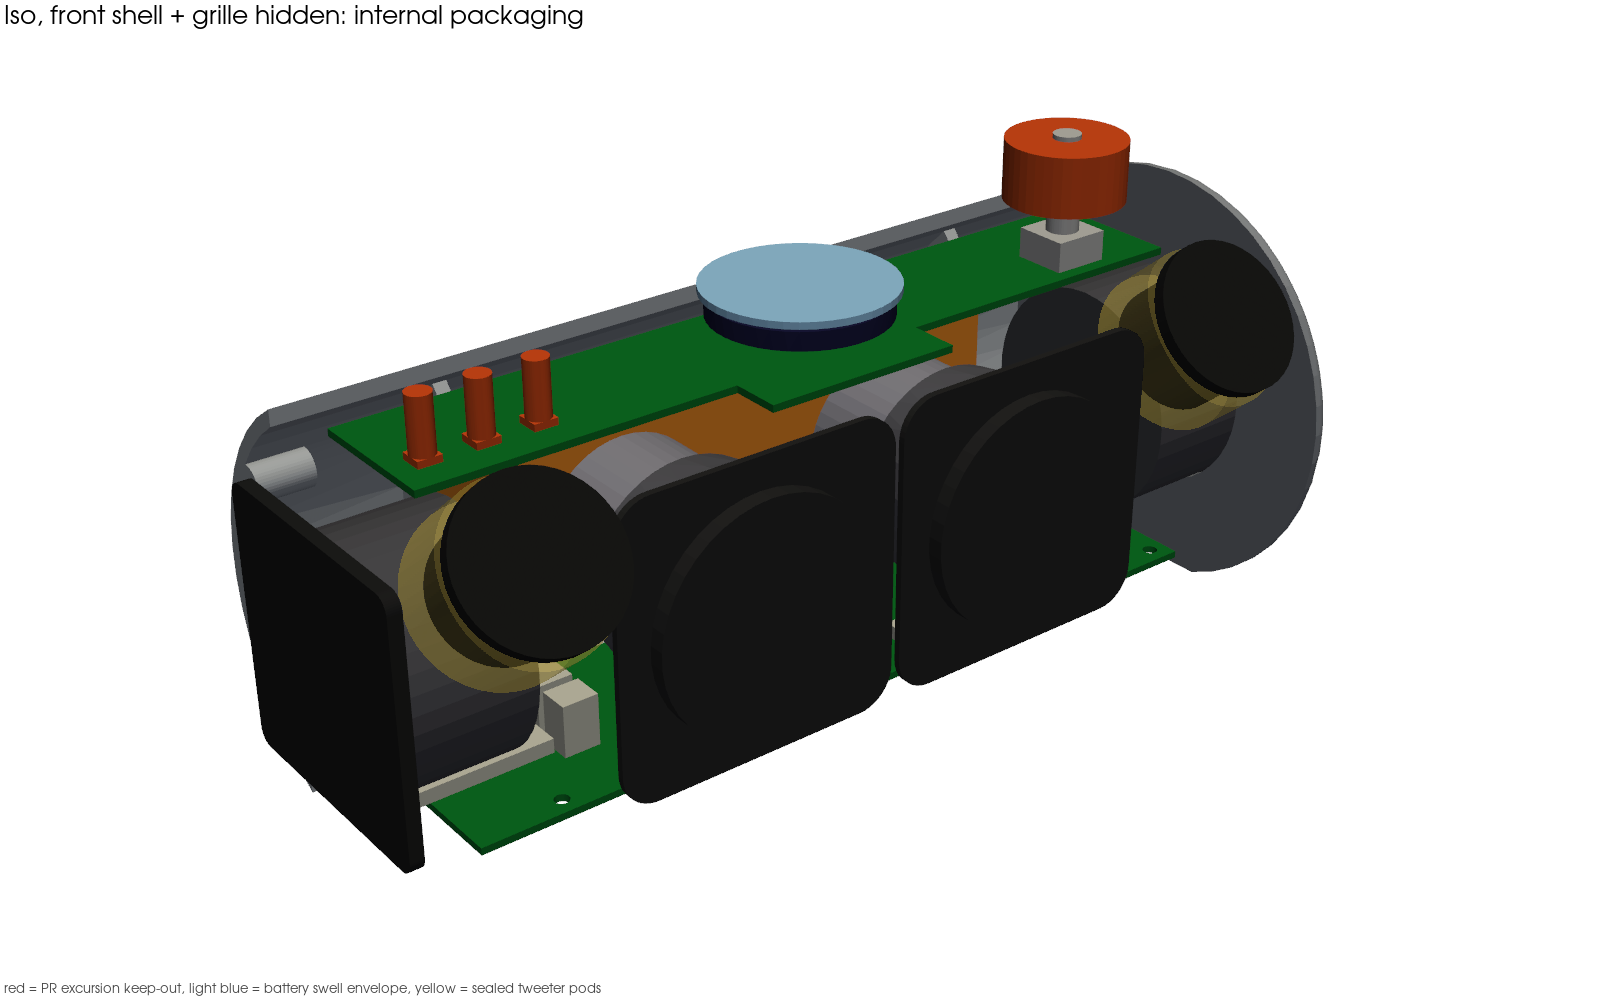
\includegraphics[width=\linewidth]{view_iso_internals.png}
\caption{Front shell and grille hidden: the two woofers rear-mounted \qty{2}{\milli\metre} apart, the UI board under the top, the main board on the floor and the battery behind the woofer motors.}
\end{subfigure}\\[4pt]
\begin{subfigure}[t]{0.49\linewidth}\centering
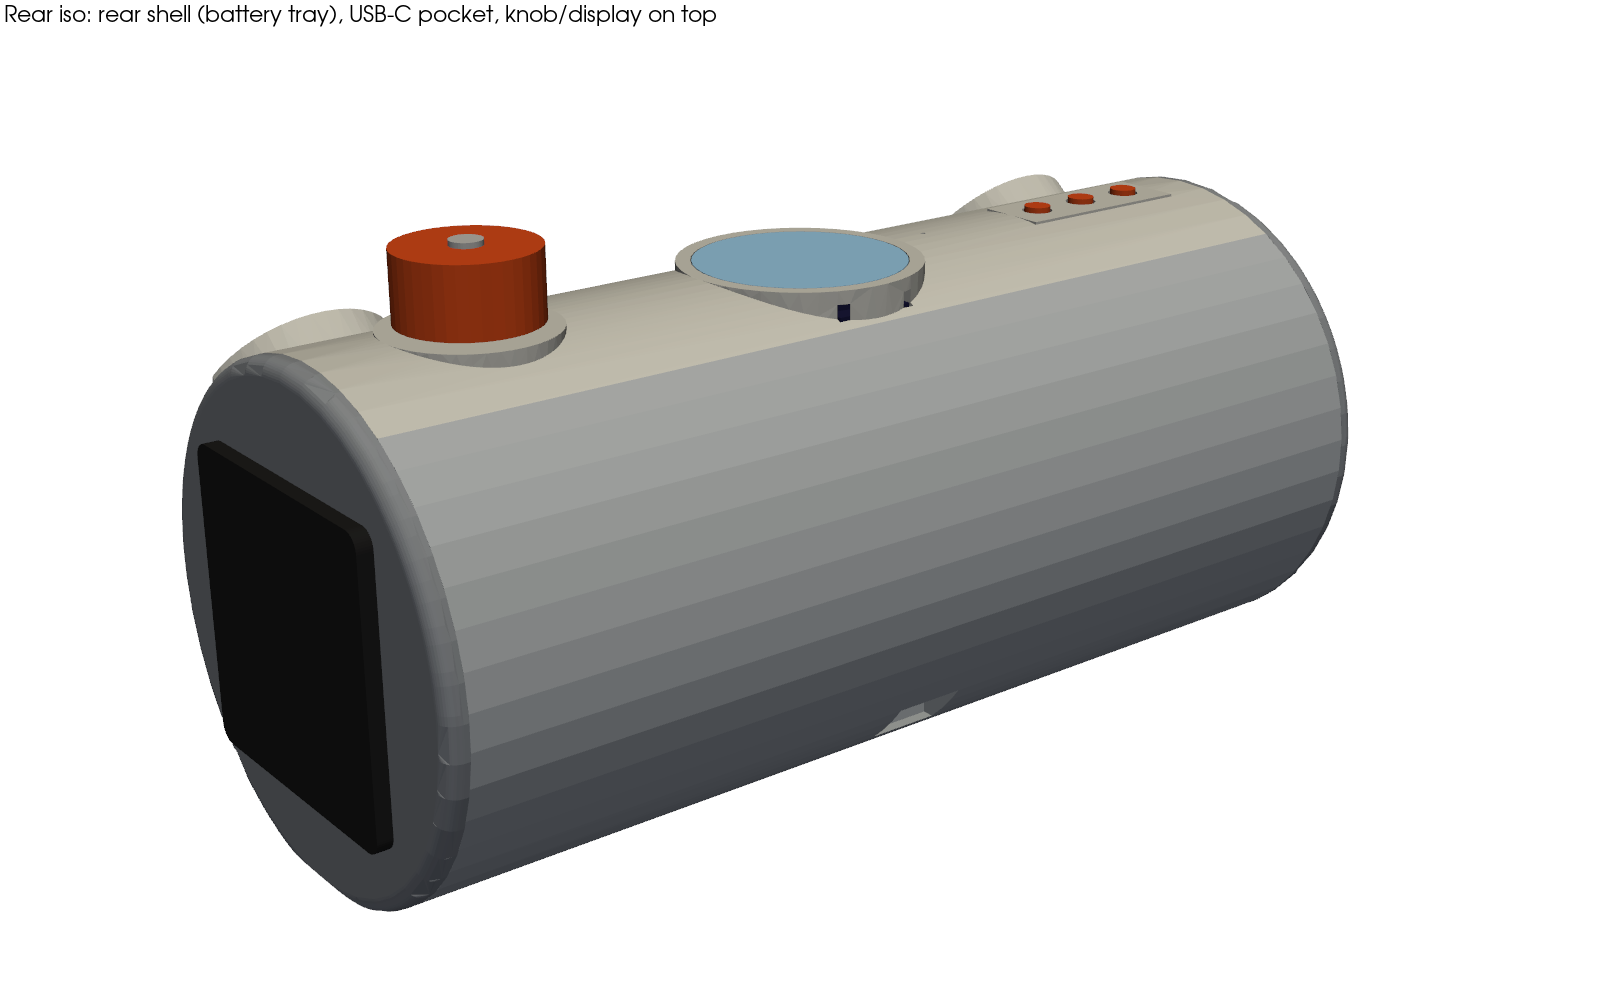
\includegraphics[width=\linewidth]{view_iso_rear.png}
\caption{Rear iso: the shell seam and the USB-C pocket at the bottom centre.}
\end{subfigure}\hfill
\begin{subfigure}[t]{0.49\linewidth}\centering
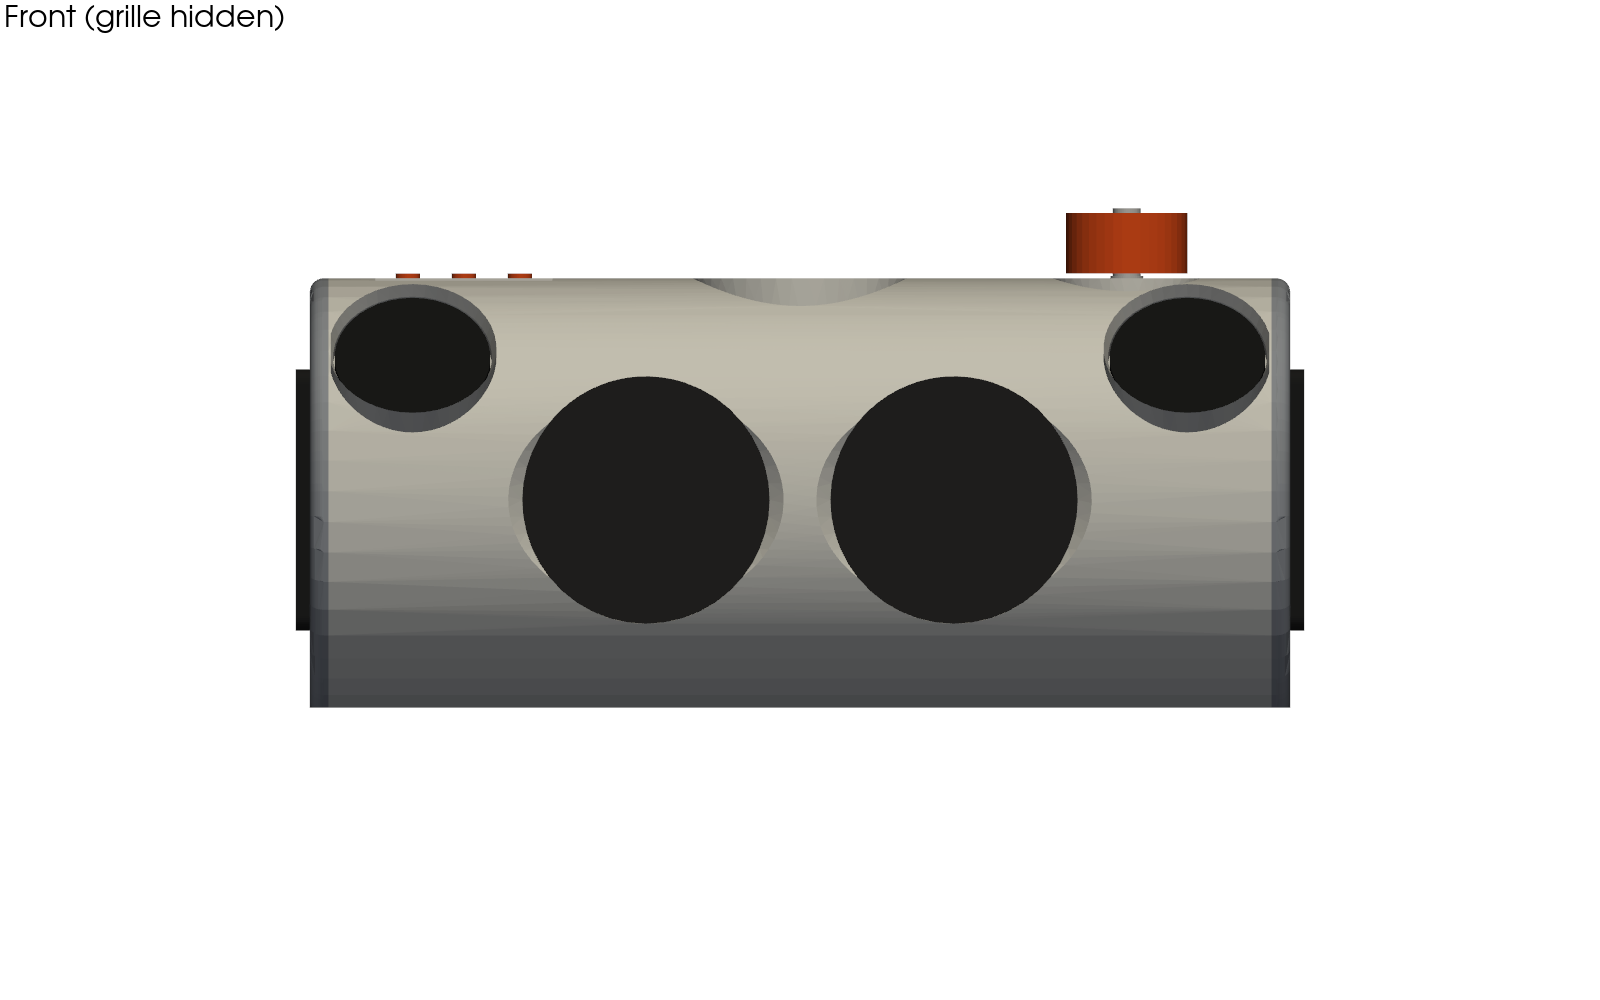
\includegraphics[width=\linewidth]{view_front.png}
\caption{Front: woofer openings \qty{66}{\milli\metre} apart, tweeters \qty{166}{\milli\metre} apart.}
\end{subfigure}
\caption{Concept CAD views. The overall envelope is \qtyproduct{216 x 95 x 92}{\milli\metre}; the knob adds \qty{14}{\milli\metre} on top. In the internal view, red marks the PR excursion keep-outs, light blue the battery swell envelope and yellow the sealed tweeter pods.}
\label{fig:cad-views}
\end{figure}

\begin{figure}[htbp]
\centering
\begin{subfigure}[t]{0.32\linewidth}\centering
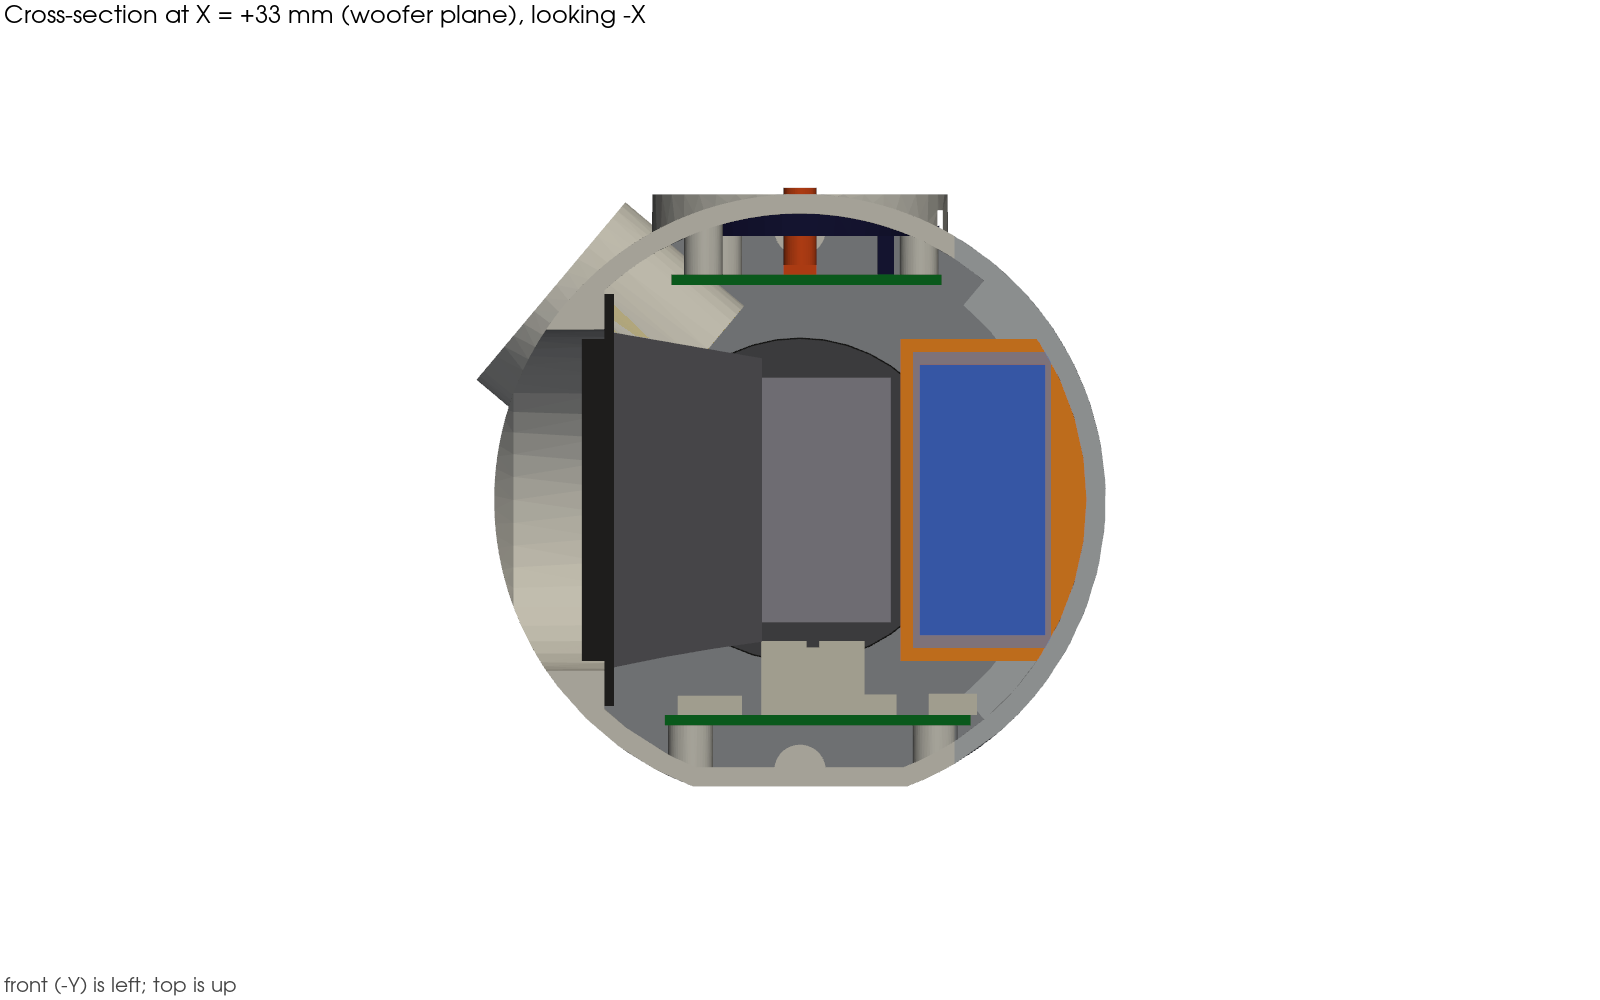
\includegraphics[width=\linewidth]{view_section_xp33_woofer.png}
\caption{Section at $x=\qty{+33}{\milli\metre}$ (woofer).}
\end{subfigure}\hfill
\begin{subfigure}[t]{0.32\linewidth}\centering
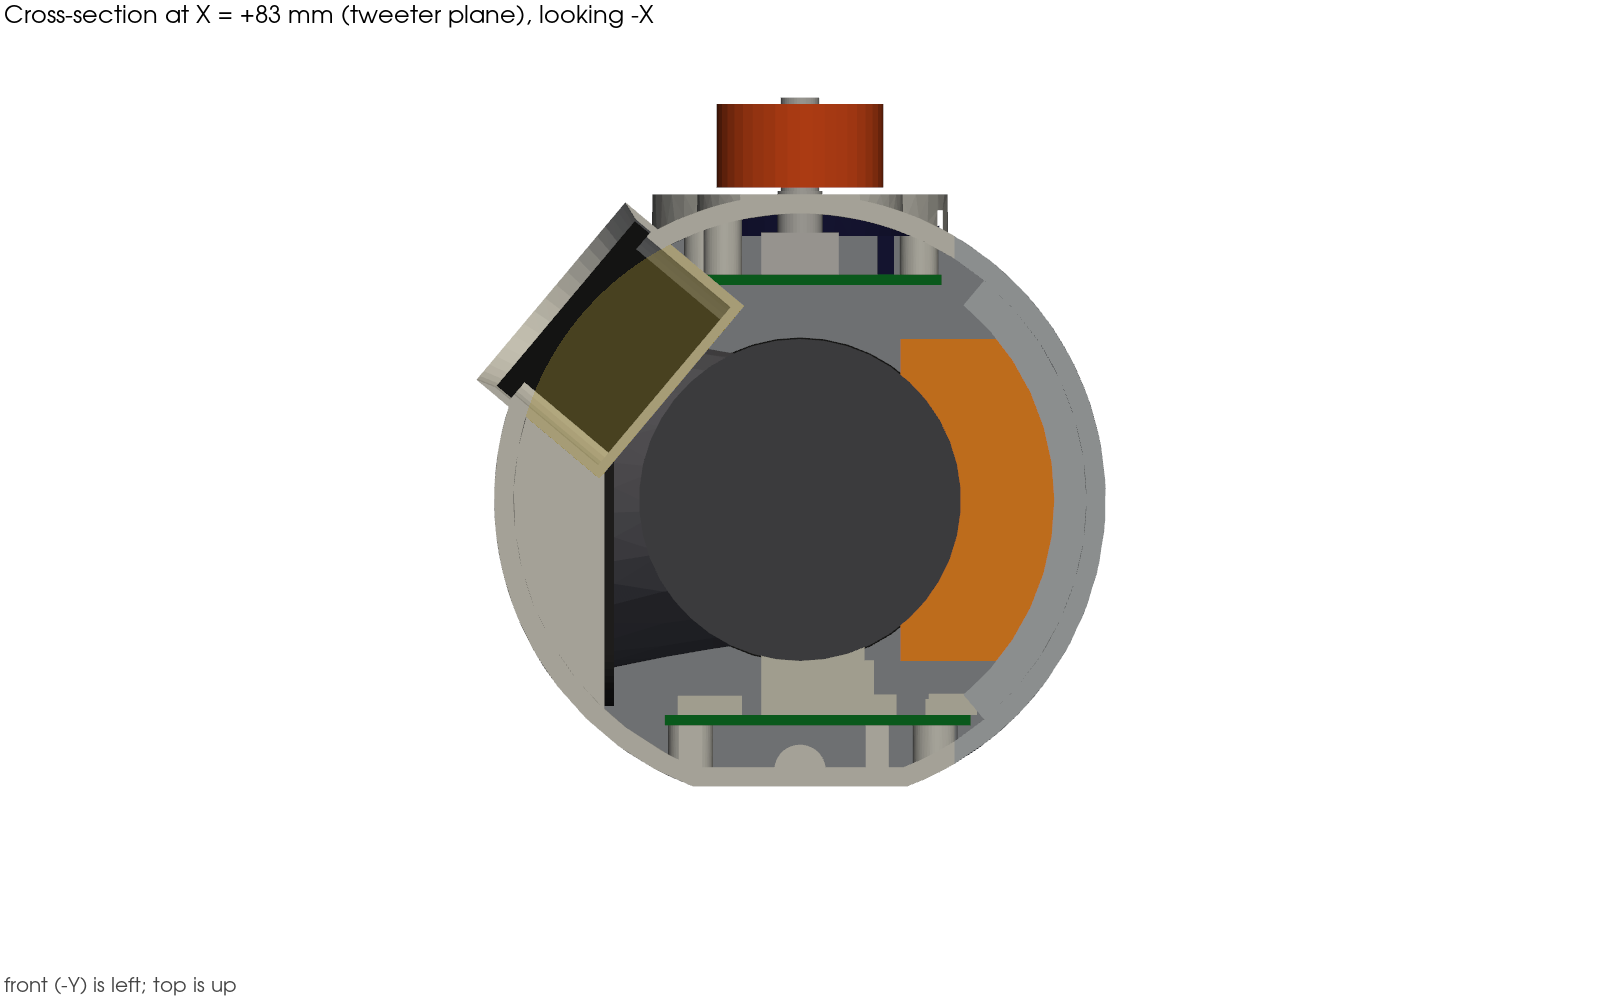
\includegraphics[width=\linewidth]{view_section_xp83_tweeter.png}
\caption{Section at $x=\qty{+83}{\milli\metre}$ (tweeter pod).}
\end{subfigure}\hfill
\begin{subfigure}[t]{0.32\linewidth}\centering
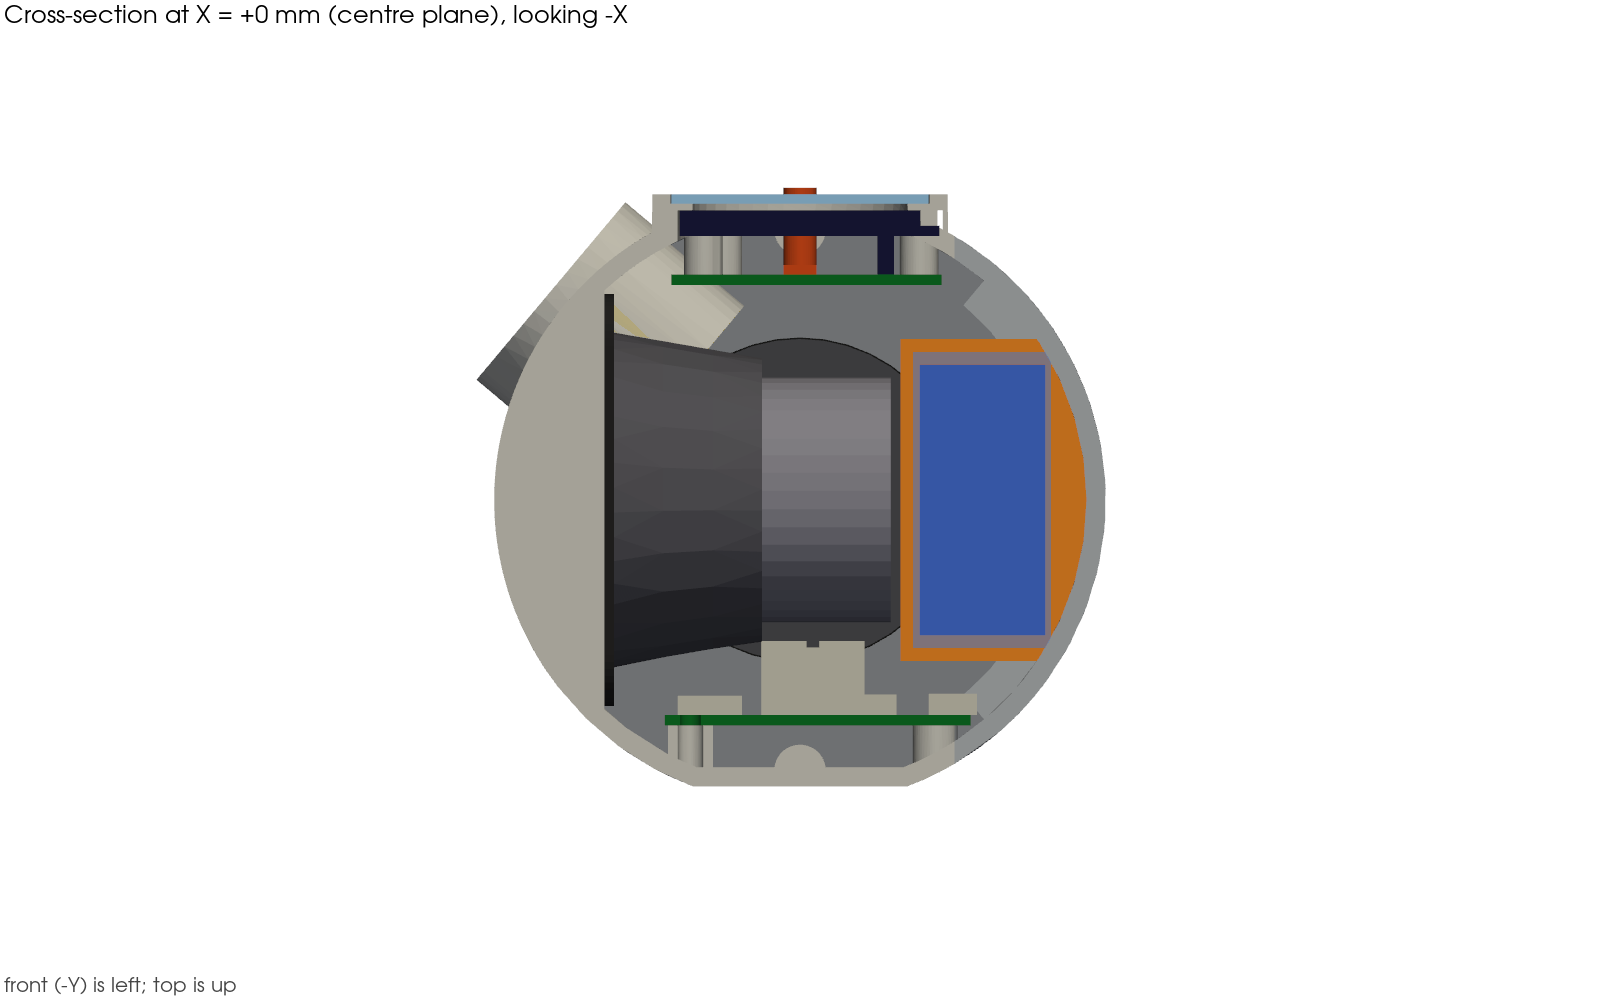
\includegraphics[width=\linewidth]{view_section_xp0_centre.png}
\caption{Section at $x=0$ (centre).}
\end{subfigure}\\[4pt]
\begin{subfigure}[t]{0.49\linewidth}\centering
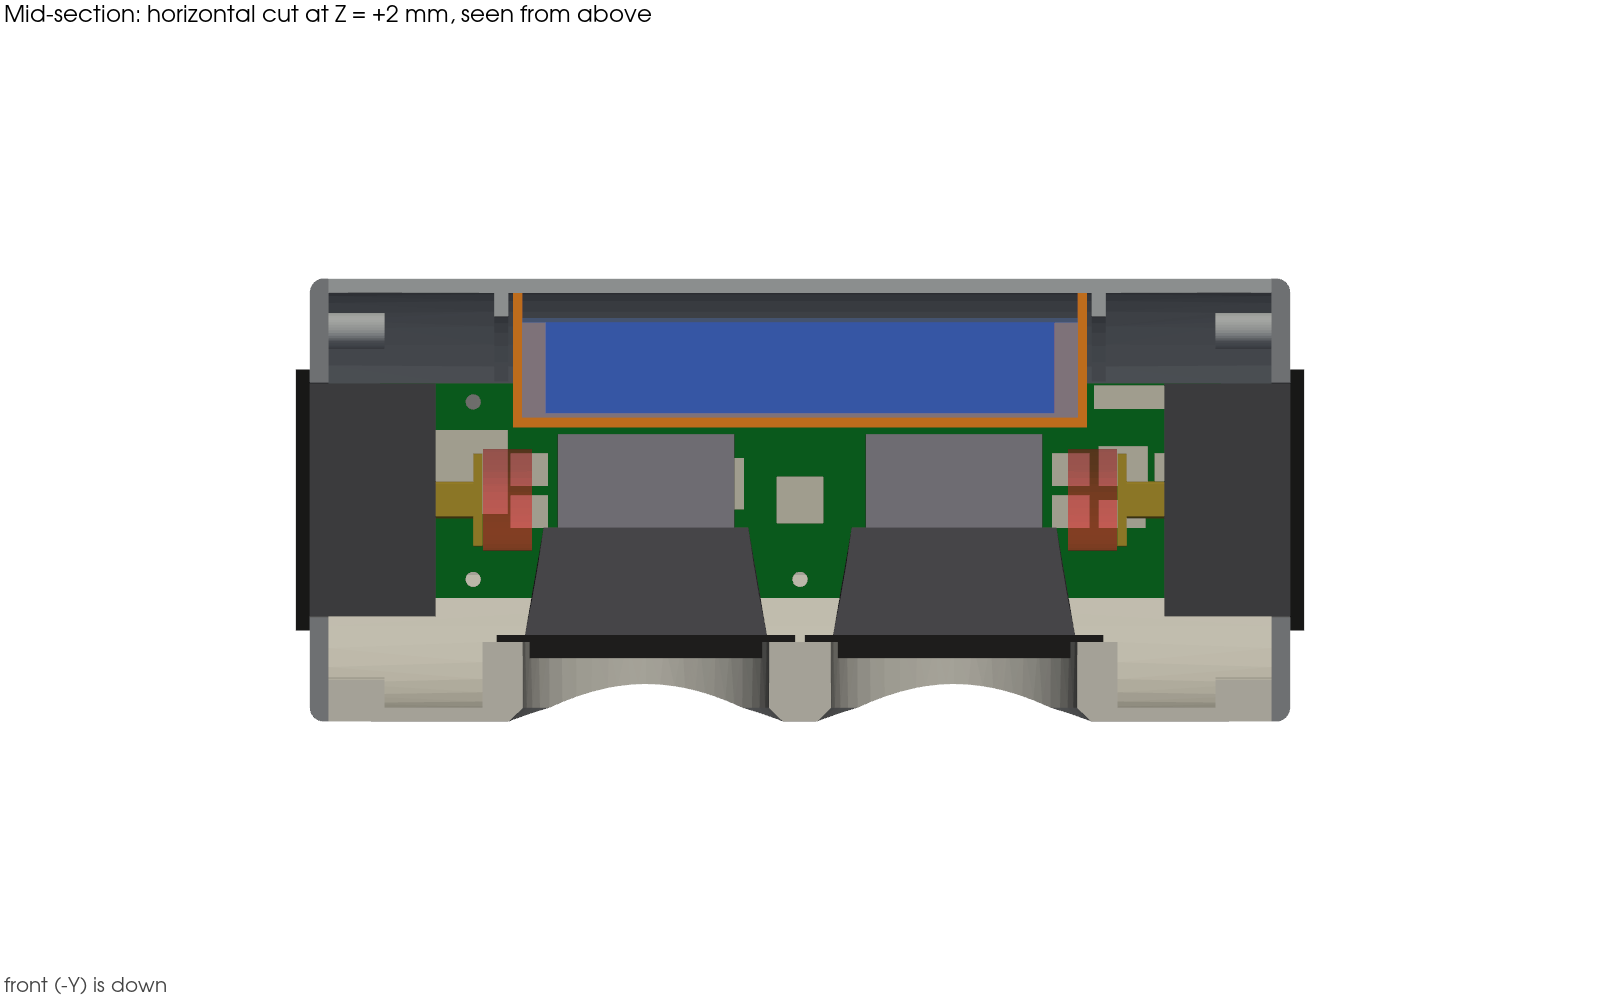
\includegraphics[width=\linewidth]{view_section_z_mid.png}
\caption{Horizontal section at mid-height.}
\end{subfigure}\hfill
\begin{subfigure}[t]{0.49\linewidth}\centering
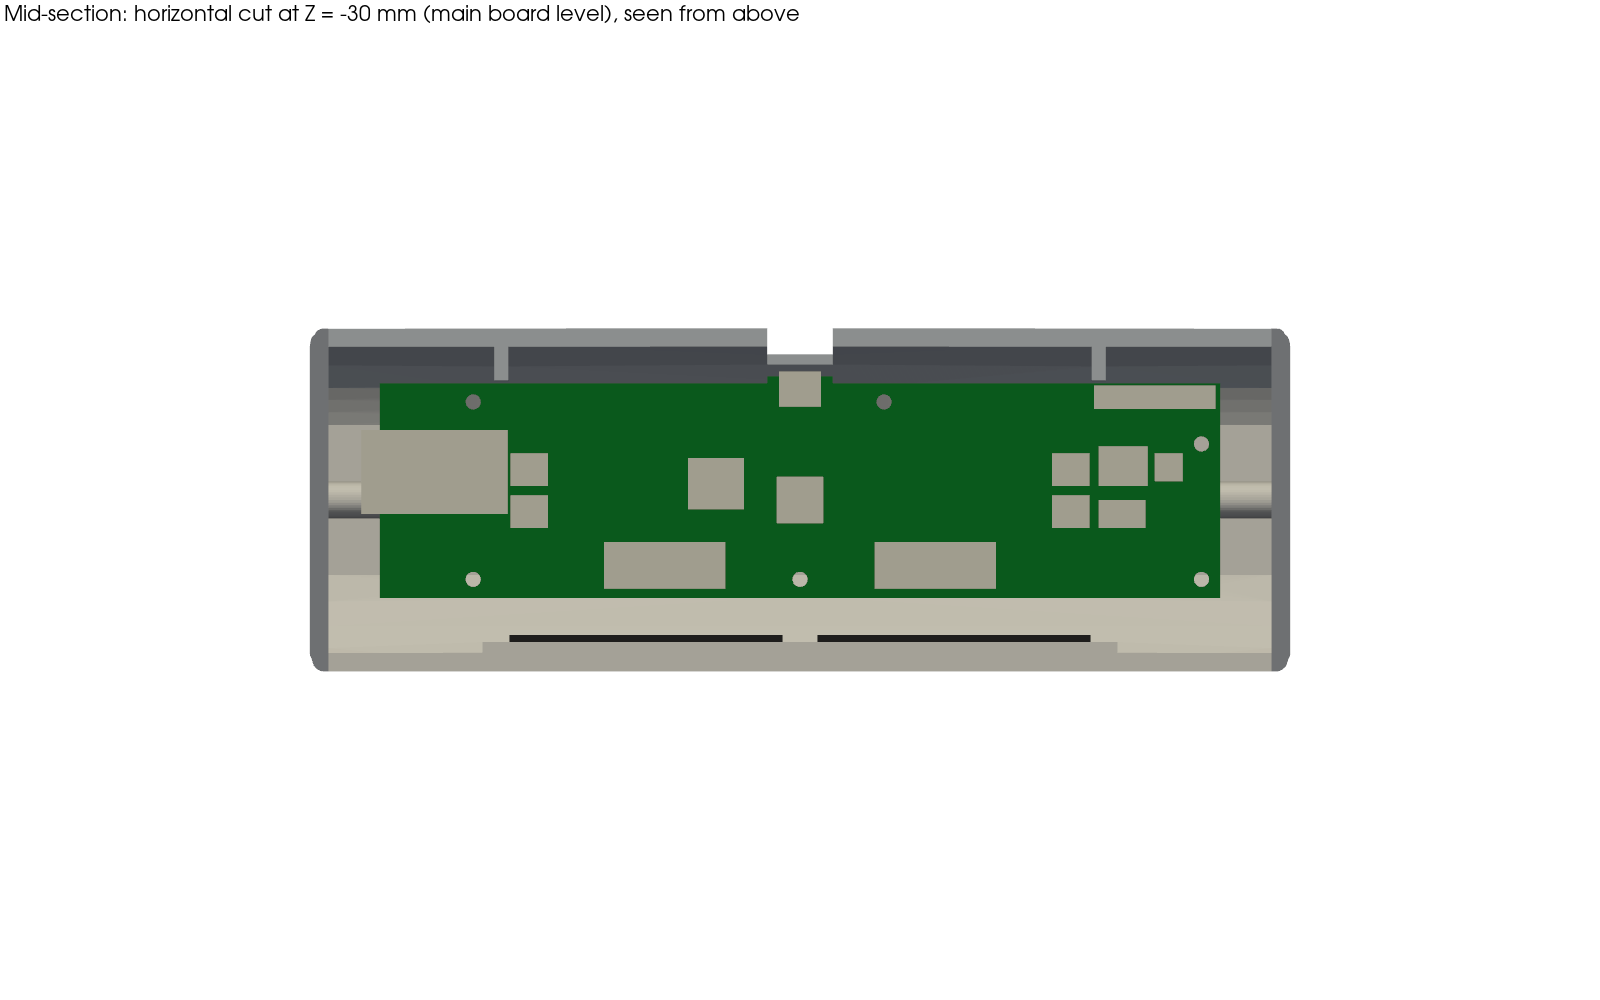
\includegraphics[width=\linewidth]{view_section_z_board.png}
\caption{Horizontal section at the main-board level.}
\end{subfigure}
\caption{Cross-sections. The woofer section shows why the diameter is \qty{95}{\milli\metre}. The ND65-8's flange sits at least \qty{30}{\milli\metre} off the axis, its \qty{48}{\milli\metre} depth eats most of the tube, and the \qty{19.5}{\milli\metre} battery fits only in the slab behind the motors. The tweeter section shows the sealed pod (Ø\qtyproduct{32 x 21.5}{\milli\metre}) squeezed between the PR basket and the skin, which is why the waveguide became a \qty{3}{\milli\metre} bezel.}
\label{fig:cad-sections}
\end{figure}

\subsection{Net volume}

\begin{table}[htbp]
\centering\small
\caption{Net internal volume from the model's solids. Open-frame parts use fill factors: \num{0.25} for the woofer basket and \num{0.2} for the PR basket. Source: \protect\src{docs/mech_envelope.md} §5.}
\label{tab:volume}
\begin{tabular}{@{}l S[table-format=4.1]@{}}
\toprule
Item & {cm\textsuperscript{3}} \\
\midrule
Gross tube interior (Ø89 $\times$ \qty{202}{\milli\metre}, flat floor) & 1243.6 \\
Shell intrusions (baffle land, ribs, bosses, standoffs, pads, tray walls) & -75.8 \\
Tweeter pods (sealed, excluded) & -26.2 \\
Woofer front openings (air outside the box) & -39.3 \\
Woofers $\times$2 & -92.1 \\
PRs $\times$2 (inside portion) & -20.1 \\
Battery (nominal) & -89.3 \\
Main PCB + modelled parts & -21.3 \\
UI PCB, display, encoder, buttons & -14.6 \\
Wiring, foam, gasket allowance & -15.0 \\
\midrule
\textbf{Net box volume} & \bfseries 848 \\
\bottomrule
\end{tabular}
\end{table}

\qty{0.85}{\litre} is \qty{0.10}{\litre} more than the \qty{0.75}{\litre} the driver alignment assumed. Unmodelled board parts and the real driver shapes will cost perhaps another \qtyrange{20}{30}{\centi\metre\cubed}, so A1 uses \qty{0.82}{\litre}. The A1 what-ifs show that the extra volume is worth less than \qty{0.1}{\decibel}, so it is margin, not performance.

\subsection{Part split, fasteners and leaks}

\begin{table}[htbp]
\centering\small
\caption{Printed parts. All fit the \qtyproduct{220 x 220 x 220}{\milli\metre} build volume. The shells print standing on end, so their walls are vertical. Total shell mass is about \qty{310}{\gram} of PETG. Source: \protect\src{docs/mech_envelope.md} §3.}
\label{tab:parts}
\begin{tabularx}{\linewidth}{@{}l l >{\raggedright\arraybackslash}X@{}}
\toprule
Part & Bounding box (mm) & Contents \\
\midrule
Front shell ($y<+24$) & $202\times74\times92$ & Baffle land, tweeter pods, top UI pads and bosses, floor standoffs, seam lips \\
Rear shell ($y>+24$) & $202\times24\,(+8)\times82$ & Battery tray, which doubles as a puncture shield; rear ribs; USB-C pocket \\
End cap $\times2$ & $95\times92\times4$ (+ ribs) & PR mount (flange \qty{3}{\milli\metre} proud), spigot ring with gasket, 5 axial screws \\
Knob, plungers & small & Lens is a laser-cut acrylic or polycarbonate disc \\
Grille (not printed) & \qty{0.8}{\milli\metre} perforated Al & Rolled to $R\,\qty{48.3}{\milli\metre}$; tabs plus VHB; Ø38 holes for the tweeter bosses \\
\bottomrule
\end{tabularx}
\end{table}

The passive-radiator alignment assumes a well-sealed box, so the concept gaskets every seam and driver and seals the encoder, USB-C receptacle, buttons and microphone port. The power button SW4 sits in a recessed Ø\qty{10}{\milli\metre} pocket on the top, so a palm or bag cannot press it \src{docs/mech_envelope.md}.

\begin{checked}
The FreeCAD script checks every pair of solids for interference (none) and reports clearances. The tightest are \qty{0.5}{\milli\metre} (tweeter pod to woofer frame) and \qty{1.0}{\milli\metre} (pod to PR basket, battery to shell). Because they come from datasheet drawings, the real drivers and pack must be measured and the script re-run. The net volume is computed from the solids, with fill factors for open-frame parts. The same parameter block drives the BEM hull, whose sections match the CAD within a median of \qtyrange{0.7}{0.9}{\milli\metre}.
\end{checked}

\subsection{PCB envelopes}

\begin{figure}[htbp]
\centering
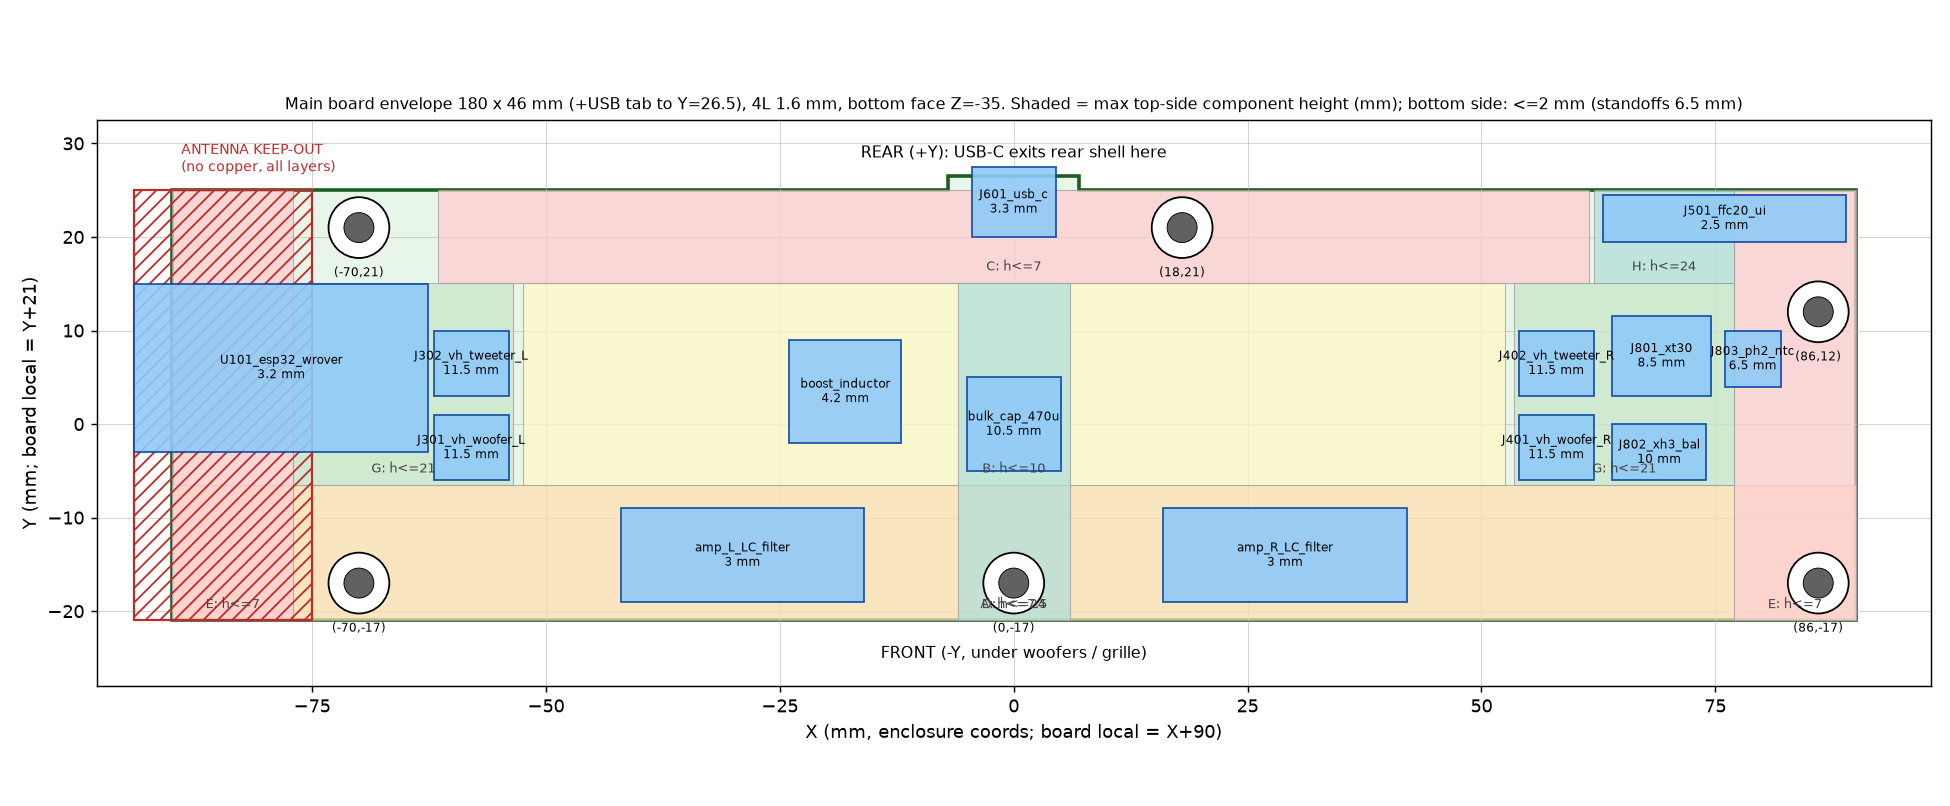
\includegraphics[width=\linewidth]{mainboard_envelope.png}
\caption{Main-board envelope: \qtyproduct{180 x 46}{\milli\metre} plus a USB-C tab, 4 layers, six M3 holes. Each height zone is set by what sits above it: \qty{7.5}{\milli\metre} under the woofer baskets, \qty{10}{\milli\metre} under the motors, \qty{24}{\milli\metre} in the centre for the \qty{470}{\micro\farad} capacitor, \qty{21}{\milli\metre} between motor and PR for the connectors. The ESP32 antenna overhangs the $-x$ edge, with no copper on any layer for $x<\qty{-75}{\milli\metre}$.}
\label{fig:mainboard-env}
\end{figure}

\begin{figure}[htbp]
\centering
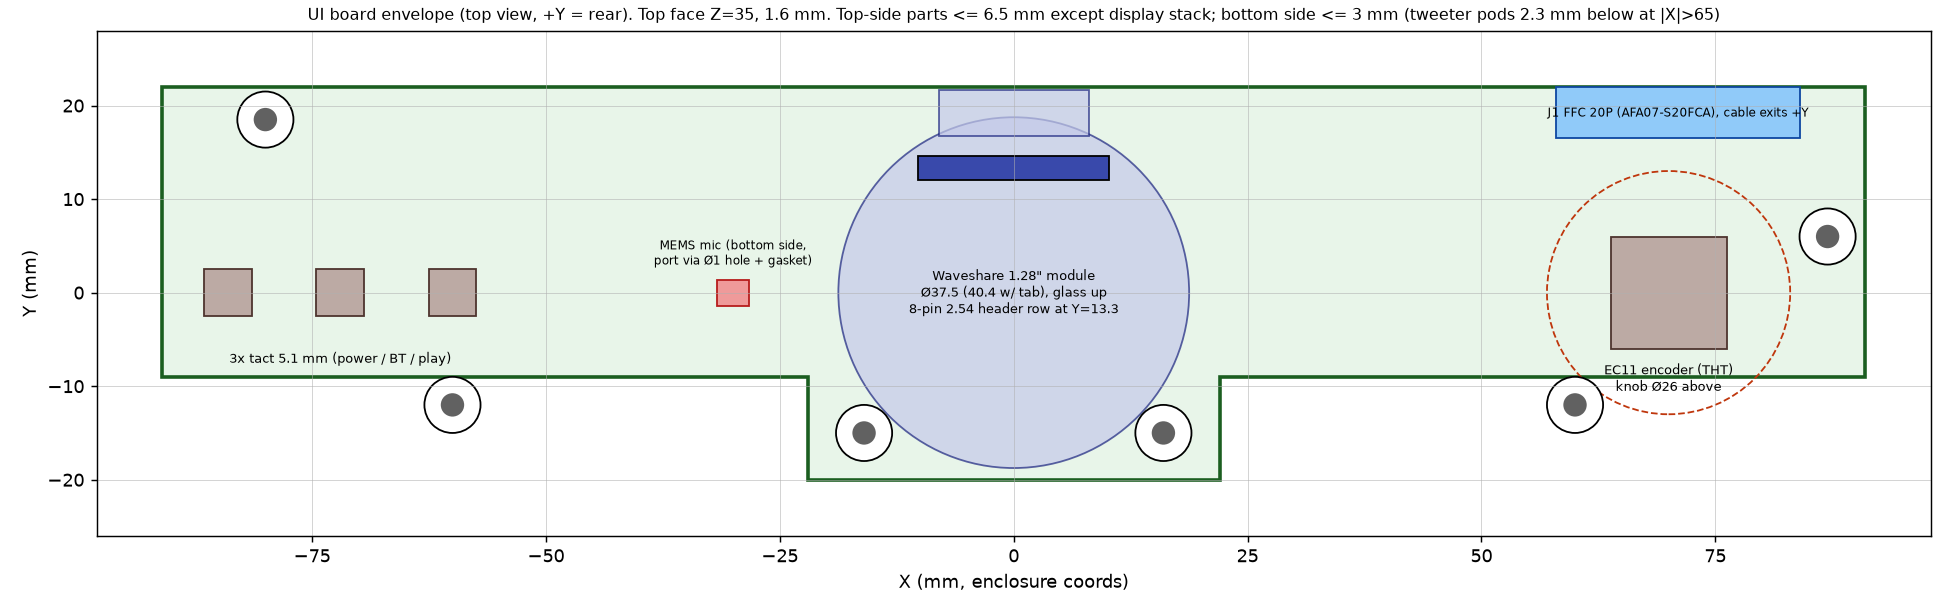
\includegraphics[width=\linewidth]{uiboard_envelope.png}
\caption{UI-board envelope: \qtyproduct{182 x 31}{\milli\metre} with a paddle under the display. It holds the display at $x=0$, the encoder at $x=\qty{+70}{\milli\metre}$, three buttons at $x=-60/-72/\qty{-84}{\milli\metre}$, the bottom-port microphone at $x=\qty{-30}{\milli\metre}$, and the FFC connector at the rear-right. The FFC runs about \qty{90}{\milli\metre} down the inside wall to J501.}
\label{fig:uiboard-env}
\end{figure}
